% https://tex.stackexchange.com/questions/36812/isnt-there-any-other-way-of-doing-double-quotes-in-latex-besides


\documentclass{beamer}

\usepackage{wx672cjk}
\usepackage[utf8]{inputenc}
\usetheme{Madrid}
\usecolortheme{beaver}
\usepackage[labelformat=empty]{caption}
\usepackage{color}
\newcommand{\quotes}[1]{``#1''}


\usepackage{hyperref}
\hypersetup{
    colorlinks=true,
    linkcolor=blue,
    filecolor=magenta,      
    urlcolor=cyan,
  }

  
 
\urlstyle{same}
 
 
%Information to be included in the title page:
\title[\emph{ACM-ICPC}] %optional
{Programming with Funny}

\subtitle{A Problem about Happy}

\author[Qiyuan, Pu] % (optional)
{Qiyuan Pu\\ 蒲启元}



\institute[SWFU] % (optional)
{
  School of Big Data and Intelligence Engineering\\
  Southwest Forestry University
}

\date[Programming Discussion 2018] % (optional)
{Online Judge System, May 2018}

\logo{
\includegraphics[height=1.3cm]{./img/icpclogo_big.png}}

%End of title page configuration block
%------------------------------------------------------------


%------------------------------------------------------------
%The next block of commands puts the table of contents at the 
%beginning of each section and highlights the current section:

\AtBeginSection[]
{
  \begin{frame}
    \frametitle{Table of Contents}
    \tableofcontents[currentsection]
  \end{frame}
}
%------------------------------------------------------------

 
 
\begin{document}
 
%The next statement creates the title page.
\frame{\titlepage}


%---------------------------------------------------------
%This block of code is for the table of contents after
%the title page
\begin{frame}
\frametitle{Table of Contents}
\tableofcontents
\end{frame}
%---------------------------------------------------------

\section{What do you live for}
%Highlighting text
\begin{frame}
  \frametitle{What do you live for}

  \begin{figure}
    \centering
    \begin{minipage}{0.45\textwidth}
        \centering
        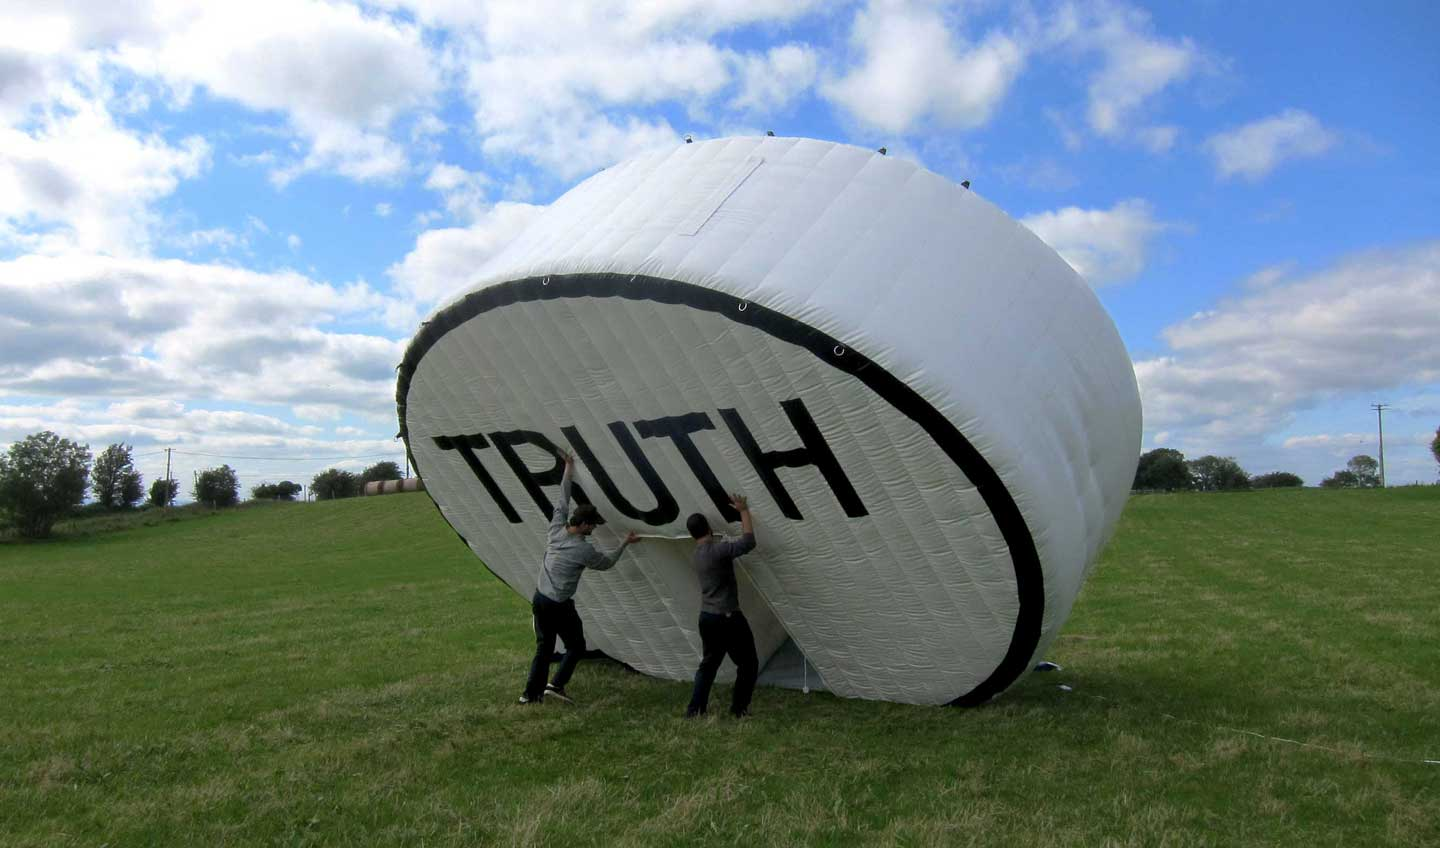
\includegraphics[width=.7\textwidth]{./img/Truth.jpg} % first figure itself
        \caption{Truth}
        \label{fig:sit-one}
    \end{minipage}\hfill
    \begin{minipage}{0.45\textwidth}
      \centering
      
\includegraphics[width=.7\textwidth]{./img/dream.jpeg} 
      \caption{Dream}
      \label{fig:sit-three}
    \end{minipage}\hfill
    \begin{minipage}{0.45\textwidth}
      \centering
      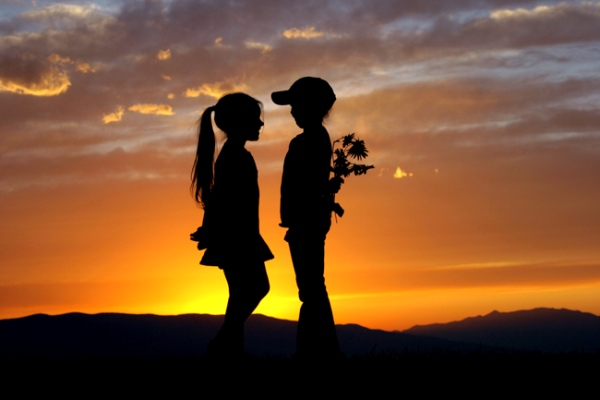
\includegraphics[width=.7\textwidth]{./img/love.jpg} 
      \caption{Love}
      \label{fig:sit-two}
    \end{minipage}\hfill
    \begin{minipage}{0.45\textwidth}
      \centering
      
\includegraphics[width=.7\textwidth]{./img/money.jpg} 
      \caption{Money}
      \label{fig:sit-four}
    \end{minipage}
    % \caption{}
    

    \textcolor{red}{What else...}
  \end{figure}
\end{frame}
  
\begin{frame}
  \frametitle{What do you live for}
  \begin{center}
    \huge {Basically, those can be reasons}
  \end{center}
  \begin{figure}
    
\includegraphics[scale=1.3]{./embed/whyHappy.pdf}
  \end{figure}
\end{frame}

\begin{frame}
  \frametitle{What do you live for}
  \begin{alertblock}{Why happy}
    \begin{enumerate}
    \item Live longer\href{http://happyproject.in/message/advantage-happy/}{(source)}
    \item More healthy\href{http://happyproject.in/message/advantage-happy/}{(source)}
    \item Marriages more succeed\href{http://happyproject.in/message/advantage-happy/}{(source)}
    \item Make more
      money\href{https://www.inc.com/rhett-power/10-reasons-why-it-is-important-create-a-happy-workplace.html}{(source)}
    \item Life should be happy, isn't it?
    \item ......
    \end{enumerate}
  \end{alertblock}

  
  \begin{center}
    \LARGE{Let's talk about one of methods to happy}
    \huge{\textcolor{red}{Programming}}
  \end{center}
  
\end{frame}


% ---------------------------------------------------------

\section{How do you think of programming}
%Highlighting text
\begin{frame}
  \frametitle{How do you think of programming}
  \begin{center}
    \huge{May you think so...}
    \begin{figure}
      
\includegraphics[scale=.38]{./img/pain11.png}
    \end{figure}
  \end{center}
\end{frame}

\begin{frame}
  \frametitle{How do you think of programming}
  \begin{center}
    \huge{Or...}
    \begin{figure}
      
\includegraphics[scale=.25]{./img/pain2.png}
    \end{figure}
  \end{center}
\end{frame}

\begin{frame}
  \frametitle{How do you think of programming}
  \Huge {\textcolor{red}{But, it can be...}}
  
  \huge{Programming running}
  \begin{center}
    \begin{figure}
      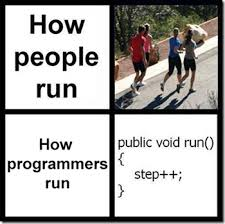
\includegraphics[scale=.6]{./img/joke1.jpeg}
    \end{figure}
  \end{center}
  
\end{frame}


\begin{frame}
  \frametitle{How do you think of programming}
  \huge{Programmer's love poem ...}
  \begin{center}
    \begin{figure}
      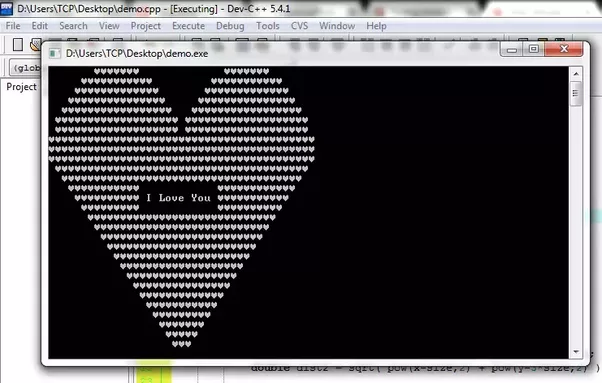
\includegraphics[scale=.3]{./img/cool_love1.png}
    \end{figure}
  \end{center}

  \huge printf(\quotes{Hello, my World});
\end{frame}


\begin{frame}
  \frametitle{How do you think of programming}
  \huge{Programmer's kids...}
  \begin{center}
    \begin{figure}
      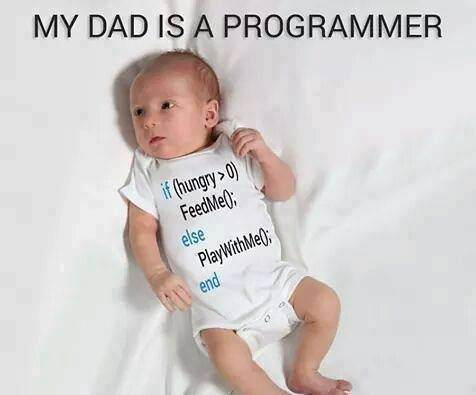
\includegraphics[scale=.4]{./img/programmer_son.jpeg}
    \end{figure}
  \end{center}

\end{frame}


\begin{frame}
  \frametitle{How do you think of programming}
  \LARGE{Why Linus is the greatest programmer}
  \begin{center}
    \begin{figure}
      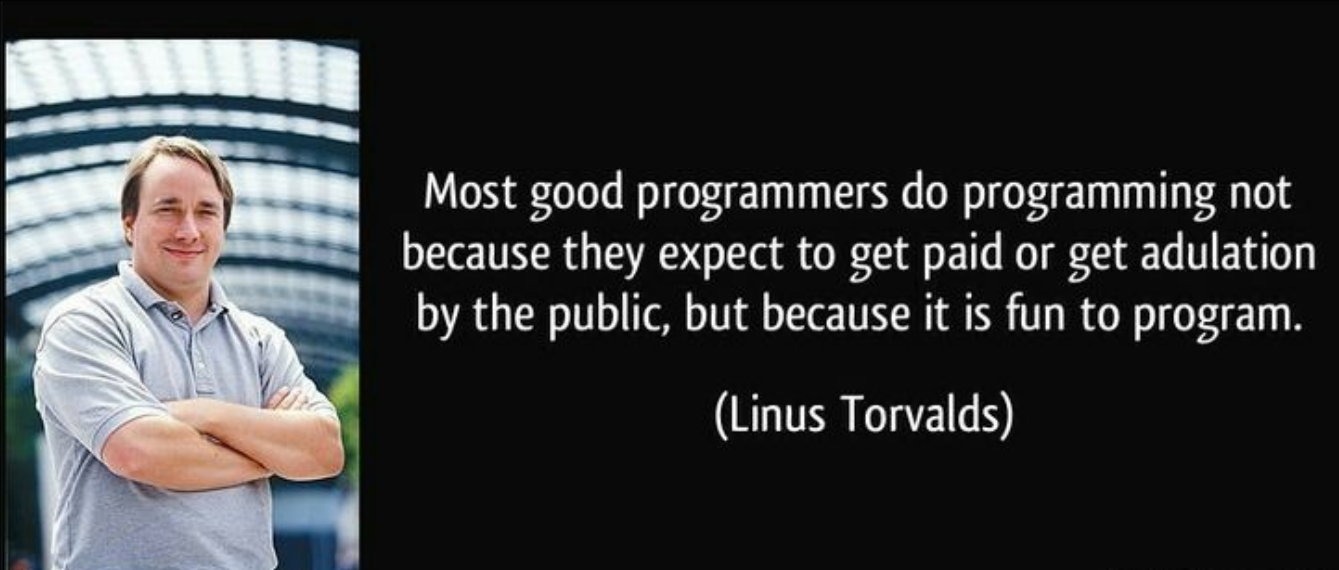
\includegraphics[scale=.22]{./img/linus.png}
    \end{figure}
  \end{center}
  \Large{But is there a way to get programming fun?}

\end{frame}


\section{Online Judge System}
%Highlighting text
\begin{frame}
  \frametitle{Online Judge System}
  \Huge{Yes, it's Online Judge System}
  \Large{An online judge is an online system to test programs in programming contests. They are also used to practice for such contests. Many of these systems organize their own contests.}

  \Huge{How it works?}
  
\end{frame}

\begin{frame}
  \frametitle{Online Judge System}
  \LARGE{Process of working}
  \begin{center}
    \begin{figure}
      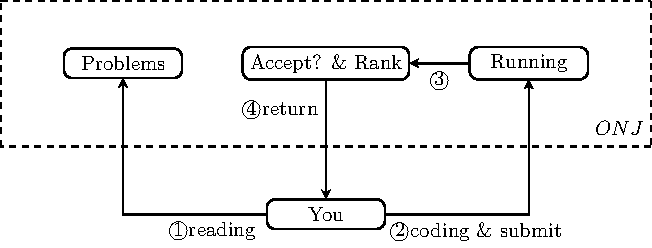
\includegraphics[scale=1.1]{./embed/online_judge.pdf}
    \end{figure}
  \end{center}
  
\end{frame}

\begin{frame}
  \frametitle{Online Judge System}
  \Huge{Some common ONJs}
  \huge International
  \begin{itemize}
  \item \href{https://www.codechef.com/}{\Large{CodeChef}}
  \item \href{https://leetcode.com/}{\Large{LeetCode}}
  \item \href{https://www.urionlinejudge.com.br/judge/en}{\Large{URI Online Judge}}
  \item \href{http://www.spoj.com/}{\Large{SPOJ}}
  \item \href{https://www.topcoder.com/}{\Large{TopCoder}}
  \end{itemize}
\end{frame}

\begin{frame}
  \frametitle{Online Judge System}
  \huge Domestic
  \begin{itemize}
  \item \href{http://www.tsinsen.com/}{\Large{清华清橙}}
  \item \href{http://poj.org/}{\Large{北大判题系统}}
  \end{itemize}
  \Huge My choice --- \href{https://www.urionlinejudge.com.br/judge/en}{URI}
  \begin{itemize}
  \item \Large{Levels}
  \item \Large{Many problems}
  \item \Large{Full functioning}
  \item \Large{English}
  \end{itemize}
\end{frame}


\section{Some example problem}
%Highlighting text
\begin{frame}
  \frametitle{Some example problem}
  \huge Problems
  \begin{itemize}
  \item \href{https://www.urionlinejudge.com.br/judge/en/problems/view/1001}{Problem 1001 --- Extremely Basic}
  \item \href{https://www.urionlinejudge.com.br/judge/en/problems/view/1002}{Problem 1002 --- Area of a Circle}
  \end{itemize}
  \huge Video Demo
  
  \Large A demo how to use URI Online Judge ---  \href{https://github.com/Puqiyuan/Latex_FIles/blob/master/acm/demo.mkv}{Video}
\end{frame}


\section{About ACM-ICPC}
%Highlighting text
\begin{frame}
  \frametitle{About ACM-ICPC}
  \Large {ACM International Collegiate Programming Contest}
  \begin{itemize}
  \item international 
  \item annual multi-tiered
  \item team competitions
  \item must be university students
  \end{itemize}
  More \href{https://en.wikipedia.org/wiki/ACM_International_Collegiate_Programming_Contest}{details}
\end{frame}


\section{Join us}
%Highlighting text
\begin{frame}
  \frametitle{Join us}
  Discussion Group
  \begin{itemize}
  \item QQ Group --- Programming SWFU(772995886)
  \item Google Group --- Programming-SWFU
  \end{itemize}
  Contact Me
  \begin{itemize}
  \item Email: pqy7172@gmail.com
  \item QQ: 1552239450
  \item WeChat: pqy7172
  \end{itemize}
  What I support
  \begin{itemize}
  \item URI usage details
  \item All beginner problems
  \end{itemize}
\end{frame}



\section{One day}
%Highlighting text
\begin{frame}
  \frametitle{One day}
  I hope one day...
\begin{itemize}
\item everyone fell in love with programming
\item we can also participate in the ACM-ICPC
\item Active discussion in the forum
  
\end{itemize}
\end{frame}


\section{Thanks}
%Highlighting text
\begin{frame}
  \frametitle{Thanks}
  \begin{center}
    \huge {\textcolor{red}{Thank you for your attention}}
    \begin{figure}
      
\includegraphics[scale=1.5]{./img/thanks.jpg}
    \end{figure}
  \end{center}
\end{frame}

  
 
\end{document}


%%% Local Variables:
%%% mode: latex
%%% TeX-master: t
%%% End:
